% arara: lualatex
\documentclass{beamer}

\begin{document}

\maketitle

\begin{frame}{We use a lot of fuels to power the world}
    \only<1,3>{
    \begin{center}
        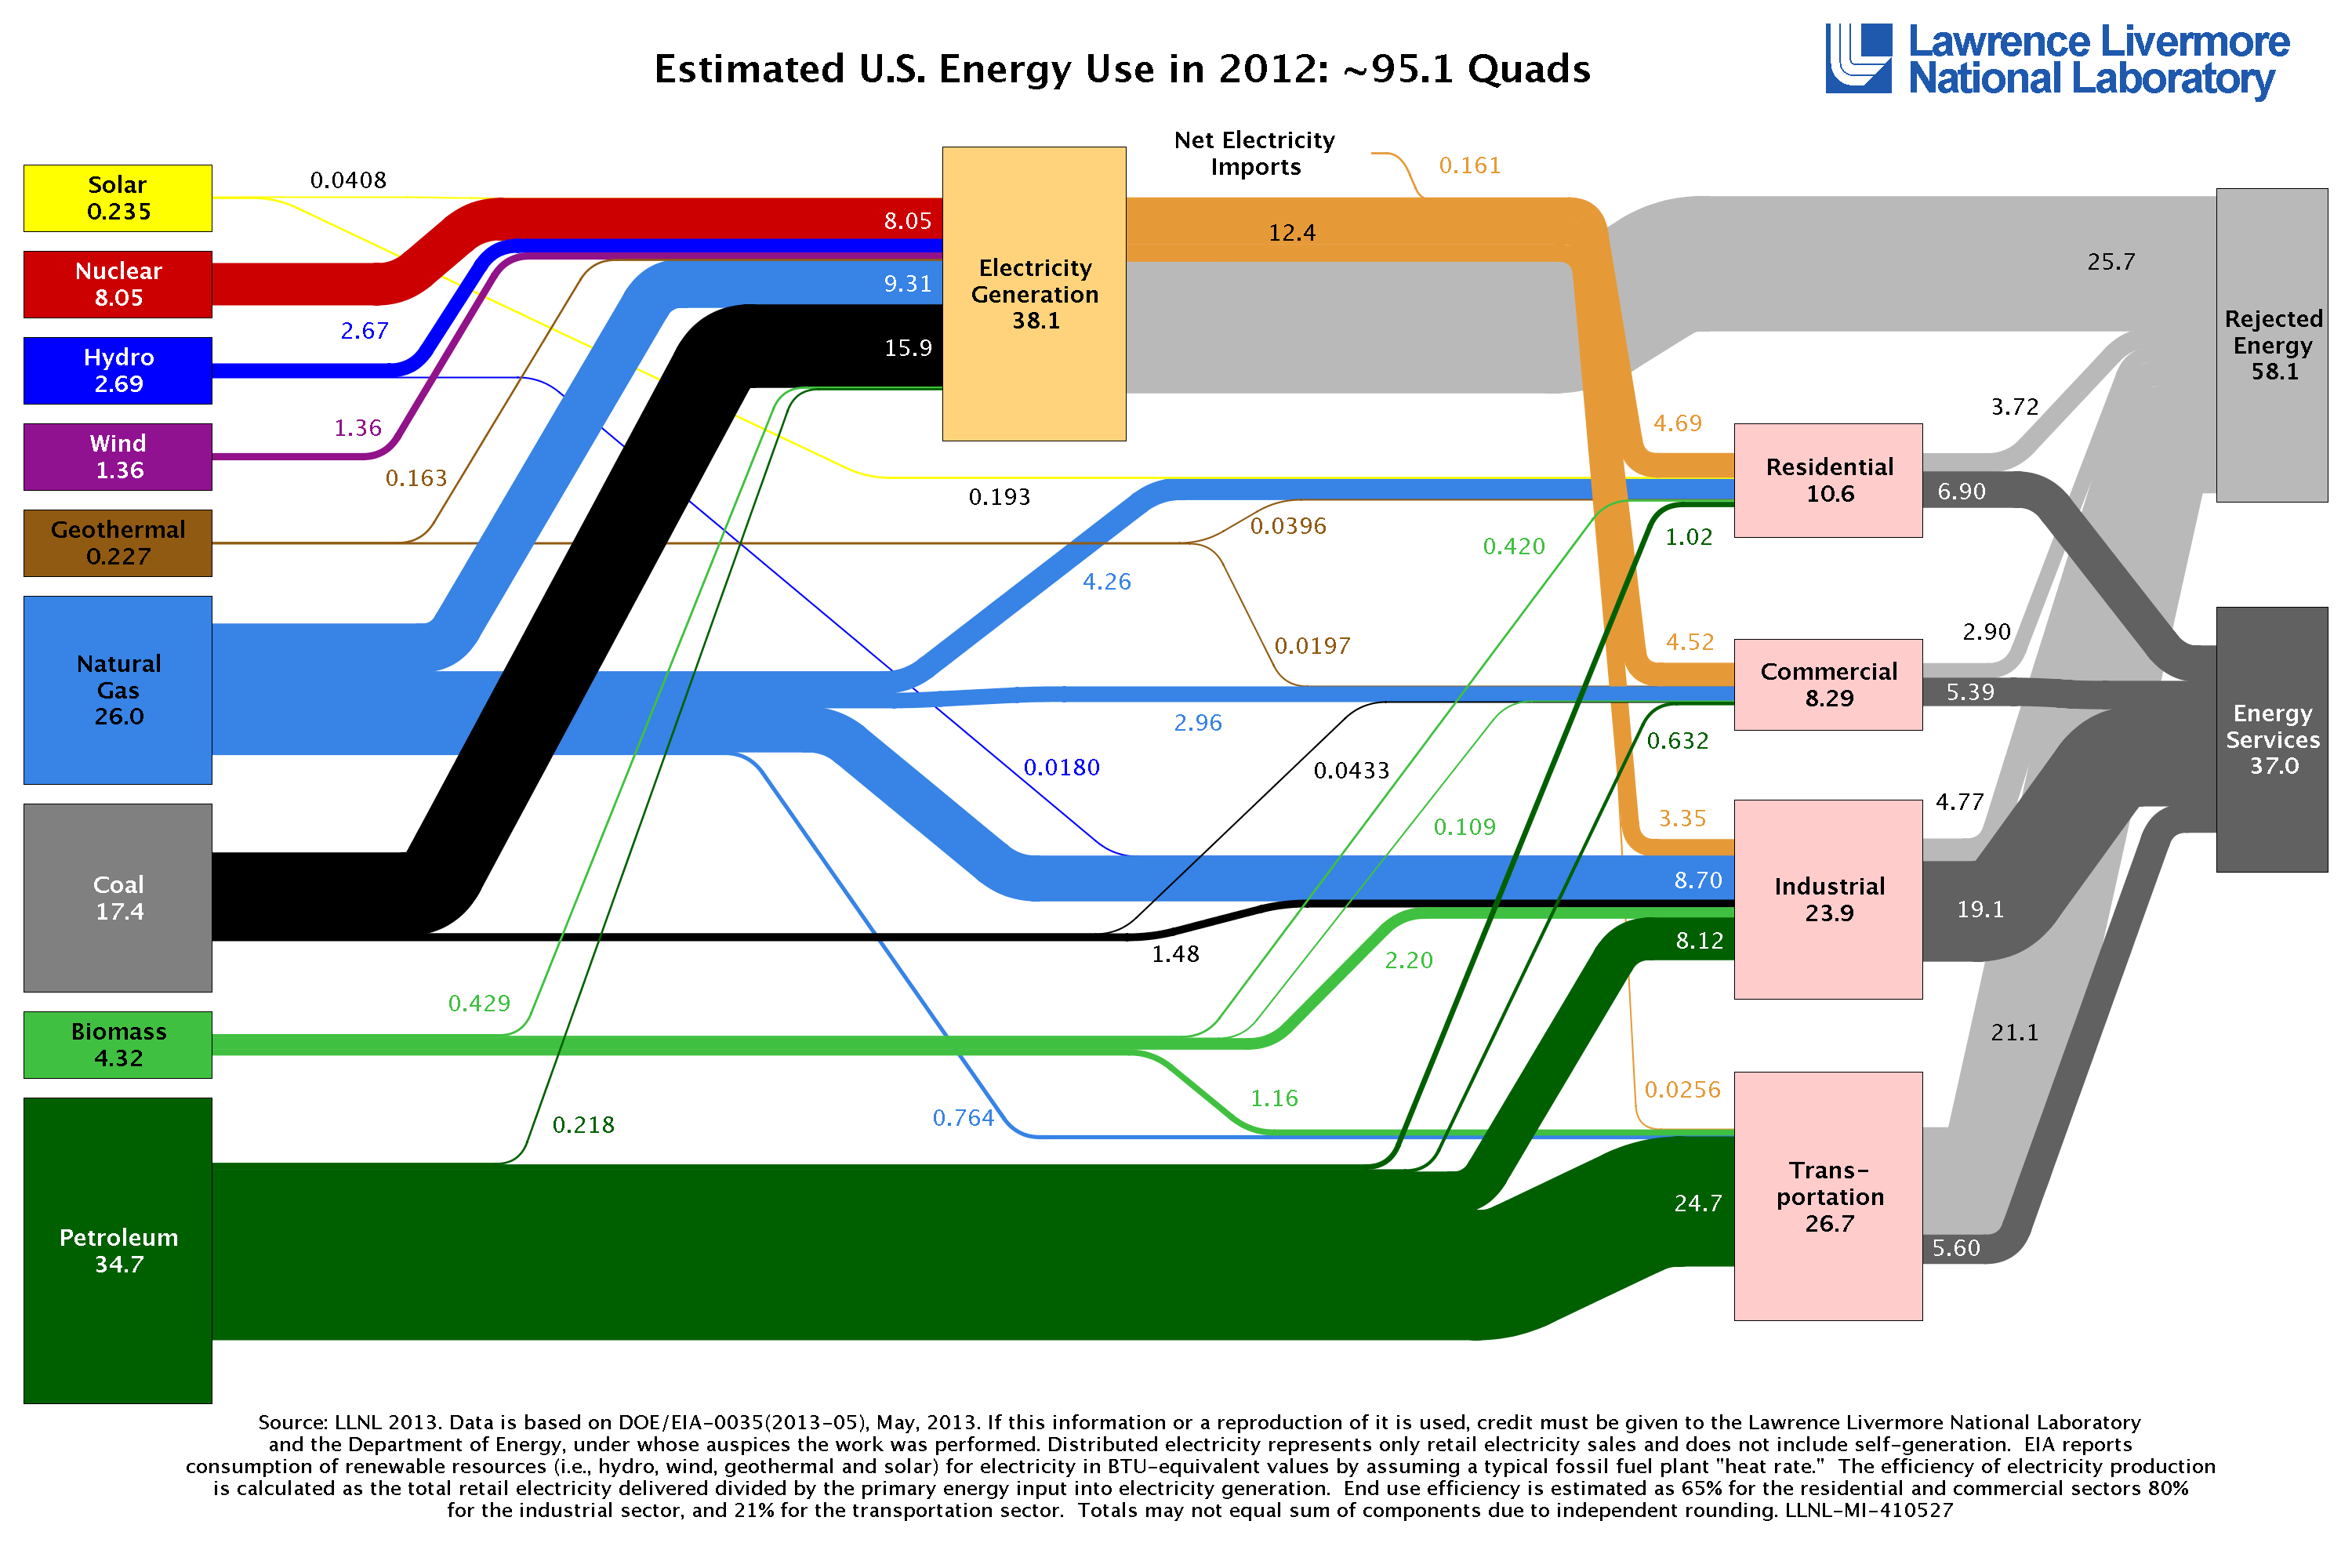
\includegraphics[width=\textwidth]{2012new2012newUSEnergy}
    \end{center}
    }
    \only<2>{Could drive to the moon and back over 150 million times in a Telsa with the amount of energy we use annually}
    % \begin{center}
        % \includegraphics[width=\textwidth]{me-to-moon}
    % \end{center}
    \only<4>{
    \begin{itemize}
        \item Combustion is predicted to remain the dominant energy conversion process for many years into the future
        \item The combustion of fossil fuels has been implicated in a number of harmful effects on human health, the environment, and the economy
        \item Two solutions have been proposed:
            \begin{itemize}
                \item Better engines
                \item Better fuels
            \end{itemize}
    \end{itemize}
    }
\end{frame}

\begin{frame}{Better engines have higher efficiency and lower emissions}
John Dec image
\end{frame}

\begin{frame}{Better fuels reduce emissions and eliminate dependence on fossil fuels}
    \begin{center}
        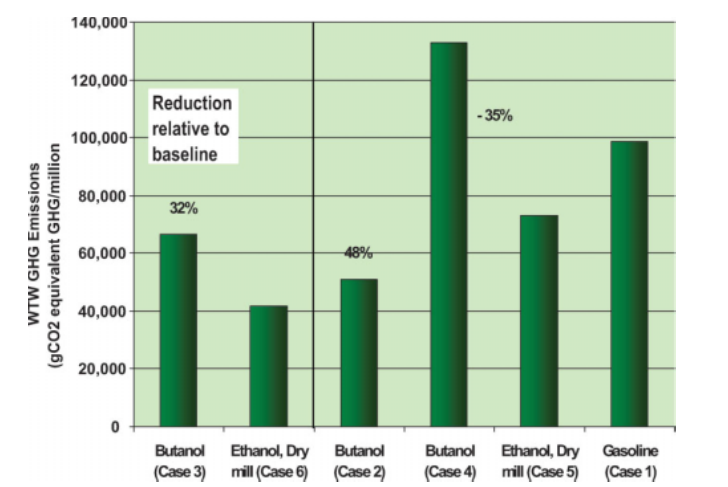
\includegraphics[width=\textwidth,height=0.85\textheight,keepaspectratio]{butanol-benefits.png}
        % \begin{tikzpicture}
        % \begin{axis}[
            % ybar,
            % scaled y ticks=false,
            % ymin=0,ymax=140000,
            % ytick={0,20000,40000,60000,80000,100000,120000,140000},
            % yticklabel style={/pgf/number format/fixed},
            % xticklabels={{Butanol\\(Case 3)}, {Ethanol Dry\\Mill (Case 6)}, {Butanol\\(Case 2)}, {Butanol\\(Case 4)}, {Ethanol Dry\\Mill (Case 5)}, {Gasoline\\(Case 1)}},
            % xticklabel style={align=center}
        % ]
        % \addplot coordinates {(1,65000) (2,42000) (3,50000) (4,132000) (5,75000) (6,98000)};
        % \end{axis}
        % \end{tikzpicture}
    \end{center}
\end{frame}

\begin{frame}{We need both solutions to make substantial progress}
    \begin{itemize}
        \item Neither solution will be able to mitigate all of the negative impacts of combustion by itself
        \item Selecting the “best” alternative fuel requires knowledge of the “best” engine, which depends on which alternative fuel is selected…
        \item Computer-aided design and modeling can be employed to make new engines fuel-flexible \alert{if} we have good models
        \item Models must be validated with experimental data acquired under engine-relevant conditions
    \end{itemize}
\end{frame}

\end{document}
